% !TeX root = ../thesis.tex
\chapter{Initial Hardware Test \& Component Verification}\label{cha:eval}
Even though the netlist was simulated and tested in the \gls{FPGA} implementation, there is no guarantee that the hardware will work out of the box.
Therefore, all bits of all components are to be tested individually to make sure there are no wiring problems which would result in bugs which are hard to pinpoint and debug.
Testing single \glspl{IC}, especially with tri-state logic, is significantly easier when incrementally adding \glspl{IC} to the \gls{PCB}.
That way one driver of a tri-state net can be verified and when adding another driver to the net, problems can be pinpointed to the new \gls{IC} because the first one was known to work correctly.
Therefore, all \glspl{IC} are placed inside sockets.
This way all resistors, \glspl{LED} and sockets can be soldered to the \gls{PCB} at once and all the \glspl{IC} can be placed in their sockets consecutively.
Another reason for using sockets is that it is easier to change an \gls{IC} if it is faulty or breaks in the future.
\section{Test Adapter}\label{sec:testAdapter}
To facilitate the testing, all control signals including clock and reset, the instruction register inputs and the \gls{ALU} results + flags are interrupted by connectors at the side of the \gls{PCB} which can connect to test adapter boards for testing.
For the debug signals that are not busses the test adapter has \glspl{LED} to display the state of the \gls{EDiC} and DIP Switches to set each debug signal to a known value.
Additionally, the main bus and ram2data bus is connected to a test adapter but not interrupted.
The test adapter has \glspl{LED} for displaying the state and a bus driver with DIP Switches.
If not testing, the connectors can be bridged with shorting connectors which short the pins from the left to the right column (except the two tri-state busses).

Testing the individual components becomes very simple this way.
For example the instruction registers:
\begin{enumerate}
  \item Set each bit of the data input individually from the test adapter
  \item Assert the \texttt{memInstrNWE} control signal (set to 0)
  \item Trigger a clock pulse
  \item Verify that the output lines equal the input set on the test adapter
\end{enumerate}
All \glspl{IC}, including the \glspl{EEPROM} and \glspl{SRAM} can be directly tested in a couple simple steps this way.

The advantage of individually testing all the bits of all \glspl{IC} is that in integration testing one can assume that the problem is not with one specific \gls{IC}.
\TODO{Insert part of a schematic of one test adapter?}
\section{Potential Complications}\label{sec:switchGlitch}
As is normal with large designs, there were some potential problems found in the \gls{EDiC} which needed fixing.
\subsection{Shifter - Carry Flag}
The detailed testing with the test adapter did reveal one bug which was not revealed in the netlist simulation because it did not occur in any simulated program.
The carry flag of a shift operation is determined by the 8 to 1 multiplexer U102 in \cref{fig:schAlu} with the first 3 bits of the bus as select bits.
The carry should always be the last bit that was shifted out of the 8 bit word.
This way, the input D1 (a0) is set as the new carry flag when shifting by 1 bit, D2 (a1) when shifting by 2 bits and so on.
However, the input D7 is connected to a7 and not a6 as it should be.
This results in a wrong carry flag when shifting by 7 bits in either direction.

In the netlist simulation this bug was not found because there was no circumstance where a value with differing bits 7 and 8 was shifted by 7 bits and the carry flag being used in the next instruction.
These kind of bugs can go undetected for a very long time and are very hard to pinpoint with a fully running \gls{CPU}.

\subsection{Clock jitter}\label{sec:eval_clock}
\begin{sidewaysfigure}[p]
  \centering
  \begin{subfigure}[b]{.45\textwidth}
    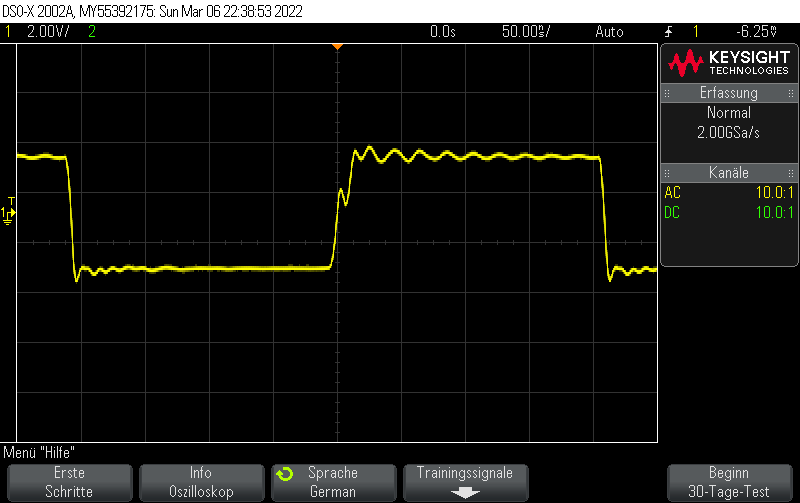
\includegraphics[width=\textwidth]{scope_0.png}
    \subcaption{No modification}
    \label{fig:clkDefault}
  \end{subfigure}%
  \hspace{.05\textwidth}
  \begin{subfigure}[b]{.45\textwidth}
    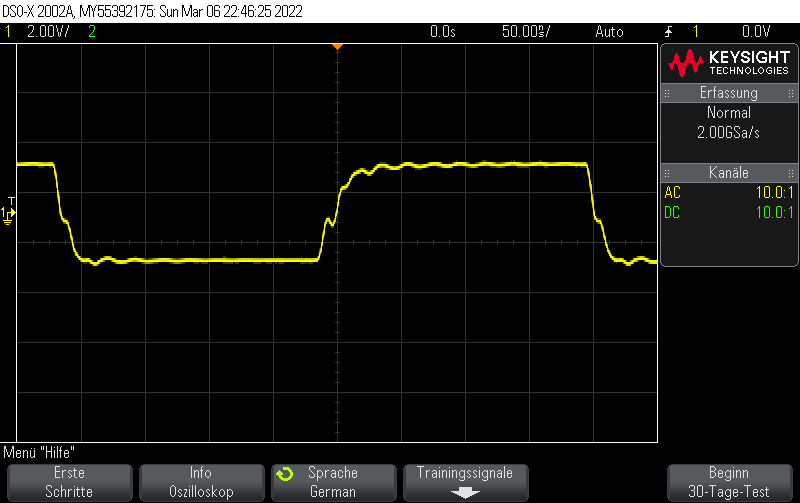
\includegraphics[width=\textwidth]{scope_2.png}
    \subcaption{R232 = \qty{33.3}{\ohm}}
    \label{fig:clk33Ohm}
  \end{subfigure}

  \begin{subfigure}[b]{.45\textwidth}
    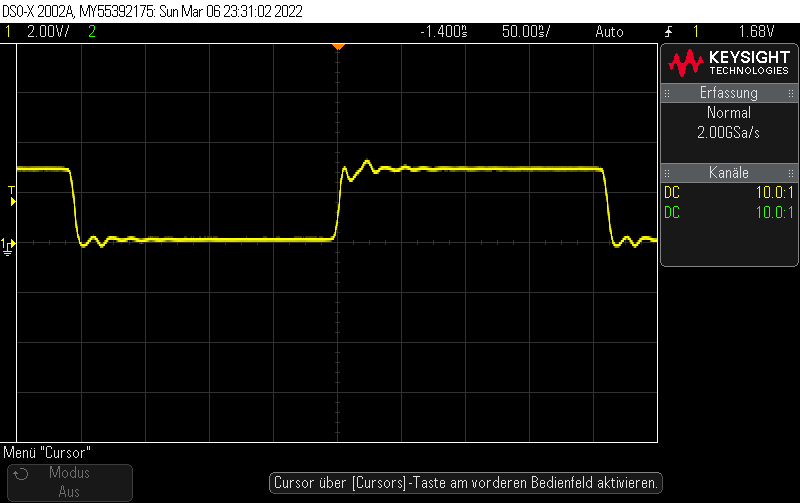
\includegraphics[width=\textwidth]{scope_3.png}
    \subcaption{R232 = \qty{0}{\ohm} and \qty{100}{\ohm} termination}
    \label{fig:clkTerm}
  \end{subfigure}%
  \hspace{.05\textwidth}
  \begin{subfigure}[b]{.45\textwidth}
    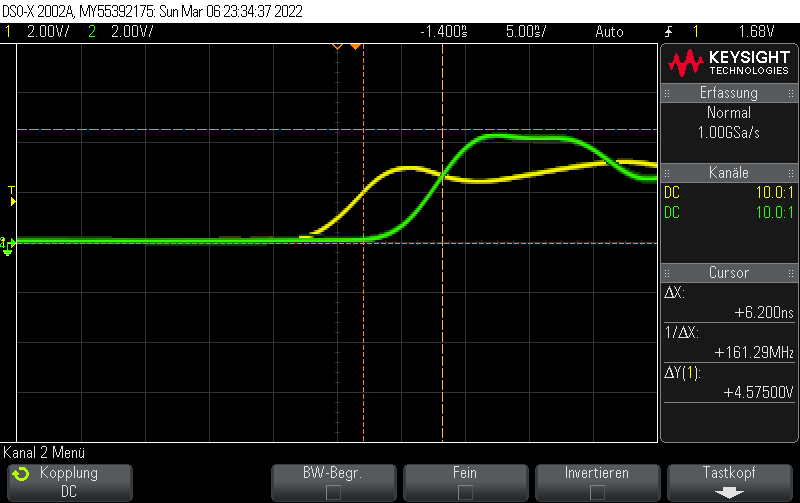
\includegraphics[width=\textwidth]{scope_7.png}
    \subcaption{Latency}
    \label{fig:clkLatency}
  \end{subfigure}
  \caption[Comparison of the clock rising edge in different configurations.]{Comparison of the rising edge of the clock in different configurations. Measured close to the clock buffer (yellow) and in \cref{fig:clkLatency} at the end of a clock lane (U204 pin 8) (green).}
\end{sidewaysfigure}
Especially with larger \glspl{PCB} a good clock distribution is a must-have.
Long clock lanes with a large load (i.e. many connected components) may induce several unwanted effects:
\begin{itemize}
  \item Jitter in the rising edge due to reflection from the ends of clock traces.
  \item A less steep rising edge due to an implicit RC-low pass filter with capacitive loads from the clock inputs and wire resistor.
  \item Over and undershoot after the edges exceeding the maximum rated voltage.
  \item Clock latency between \glspl{IC} reducing the time between two registers.
\end{itemize}
The effects must all be checked and kept under control.
The clock lane for the \gls{EDiC} was not routed as one continues trace and rather similar to a clock tree split in two.
This reduces the maximum distance one clock input is away from the clock source (U95 in \cref{fig:schClk}).
In the schematic design additional clock buffers were implemented to allow further splitting of the clock tree to help with clock distribution if it occurs and cannot be fixed other ways.

Without any modifications, the clock looked like shown in \cref{fig:clkDefault}\footnote{\cref{fig:clkDefault,fig:clk33Ohm} have AC coupling enabled which is why the y scaling is off.}.
It can be seen that there is only a little bit of overshoot but at about the middle of the rising edge there is a dip of about \qty{500}{\milli\volt}.
This could lead to a double trigger where the rising edge is detected as two individual rising edges in a register and, therefore, a counter could increment by two instead of by one.
Therefore, an attempt was made to circumvent this by changing R232 (a resistor in series after the clock buffer) from \qty{0}{\ohm} to a larger value.
In \cref{fig:clk33Ohm} a \qty{33.3}{\ohm} resistor was added.
It becomes obvious that the time constant of the implicit low-pass filter increased and with it the edge becomes less steep but the dip also becomes less of an impact.
Even though this is a decent improvement, it is not perfect.
The next attempt was to add a line termination of \qty{100}{\ohm} at the end of both clock lines instead of the \qty{33.3}{\ohm} resistor in series.
The result can be seen in \cref{fig:clkTerm}.
It shows that the dip in the rising edge is no longer there and the edge is also as steep as without any modifications.
Even though the overshoot changed a bit, it is by no means a problem and, therefore, this solution looked promising.

\Cref{fig:clkLatency} zooms into the rising edge and shows the edge at U204 pin 8 (one end of the clock tree) in green.
It can be seen that the edge looks a bit different which may be explained by the different behavior of different probes in the small time scale.
Additionally, the latency of the clock signal can be observed which is about \qty{6}{\nano\second}.
The clock frequency was chosen in \cref{sec:timing} to have a safety margin of about 30\% and, therefore, a latency of \qty{6}{\nano\second} is not a problem with a clock period of \qty{416.7}{\nano\second} (\qty{2.4}{\mega\hertz}).

\subsection{Driving Bus High}\label{sec:eval_bus}
\begin{listing}[t]
  \centering
  \begin{sublisting}[b]{.45\textwidth}
    \inputminted[linenos,
      breaklines,
      frame=leftline,
      xleftmargin=20pt,
    ]{ARM}{src/test0.s}
    \subcaption{First test program.}
    \label{lst:test0}
  \end{sublisting}

  \begin{sublisting}[b]{.45\textwidth}
    \inputminted[linenos,
      breaklines,
      frame=leftline,
      xleftmargin=20pt,
    ]{ARM}{src/test1.s}
    \subcaption{Second test program.}
    \label{lst:test1}
  \end{sublisting}%
  \hspace{.05\textwidth}
  \begin{sublisting}[b]{.45\textwidth}
    \inputminted[linenos,
      breaklines,
      frame=leftline,
      xleftmargin=20pt,
    ]{ARM}{src/test2.s}
    \subcaption{Third test program.}
    \label{lst:test2}
  \end{sublisting}
  \caption{Test programs for integration testing.}
\end{listing}
\begin{figure}[t]
  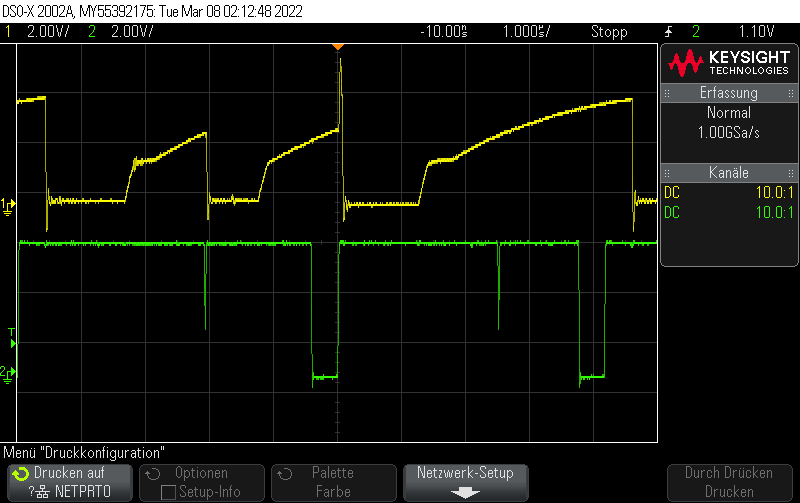
\includegraphics[width=\textwidth]{scope_9.png}
  \caption{Write Enable of \gls{MAR} register (green) and one bus lane without \texttt{0xff} driver (yellow).}
  \label{fig:busPullup}
\end{figure}
\begin{figure}[t]
  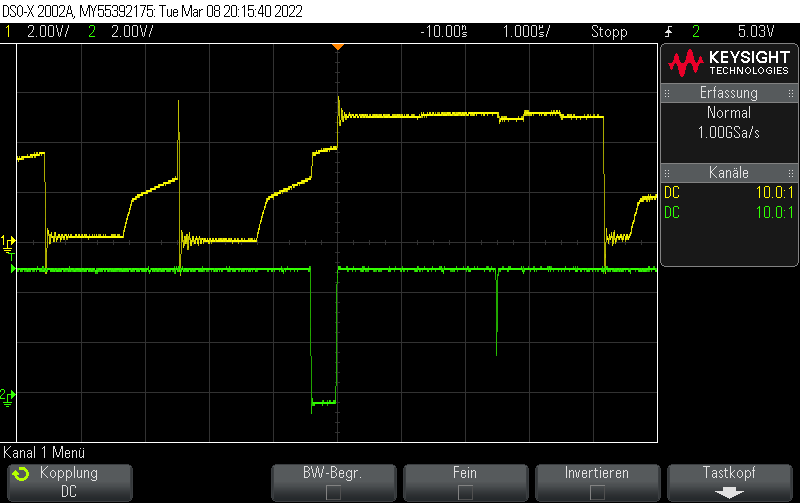
\includegraphics[width=\textwidth]{scope_10.png}
  \caption{Write Enable of \gls{MAR} register (green) and one bus lane with \texttt{0xff} driver (yellow).}
  \label{fig:busPullupFix}
\end{figure}
Until now, no program was programmed into the \glspl{EEPROM} and it was time for the first real integration test of the \gls{EDiC}.
The first program used for the integration test in \cref{lst:test0} was a basic test to see if basic instructions get executed and if the built-in I/O works.
After it ran successfully and displayed \texttt{0x42} at the displays, the second testing program from \cref{lst:test1} included the RS232 I/O extension card and its scratch register (at address \texttt{0xfe0f}).
When this also ran successfully, a more complex \gls{UART} echo program (\cref{lst:app_asm_uart}) was programmed into the \glspl{EEPROM}.
It finally had problems and did not work as expected.
It could be observed that the \gls{PC} would randomly be set to a unreasonably high value and after that \glspl{NOP} were executed until the \gls{PC} overflowed to 0 and the program started again.
However, when turning on the cycle by cycle debugger and stepping through all cycles, the program worked perfectly and bytes got read correctly from the RS232 extension card and were also sent back correctly.
After debugging for a long time, the bug was tracked down to the return instruction which sometimes (about 1 in 100 times) would return to a random instruction and not return to after the call instruction.
It was further debugged with the third test program (\cref{lst:test2}).
With an oscilloscope it was finally possible to detect the problem which is shown in \cref{fig:busPullup}.
It is actually a bug in both, the call and return instruction, which results in the same misbehavior of return to a wrong location:
Both instruction load \texttt{0xff} into the \gls{MAR} by not driving the bus with a specific value and relying on the pull-up resistors to pull the lines high.
In \cref{fig:busPullup} two \gls{MAR} write enable pulses can be seen and, especially, in the first pulse, the problem becomes apparent.
If the bus was pulled low in the cycle before the \gls{MAR} is written, the pull-up resistors take some time to pull the voltage to \qty{5}{\volt} which leaves the level at about \qty{2}{\volt} at the time of the write pulse.
This is right at the required minimum voltage to be detected as a high signal by the \emph{74F825}.
Therefore, most of the time, the register detects the bus input as a 1 but sometimes it is detected as a low signal.

The fix is quite easy as soon as the problem is detected:
A new bus driver (\emph{74F245}) is added in one of the spare slots whose A input is connected to \texttt{H1}, the B input to the bus and the output enable signal is connected to a new control signal.
This fix would have been very difficult if no output of the microcode \glspl{EEPROM} would have been free to use or if no place for spare \glspl{IC} was left on the \gls{PCB}.
Therefore, it is always important to design everything with enough resources left.

The result of the fix can be seen in \cref{fig:busPullupFix} where the bus line is raised to about \qty{3.8}{\volt} as soon as the write enable pulse starts\footnote{The even higher level on the bus line after the write enable pulse is driven by the \gls{SRAM} driver (outputs the return address in the return instruction) which is an \emph{ACT} type for compliance with the \gls{SRAM} specification. In \cref{fig:busPullup} the \gls{SRAM} probably drove a `0' to the bus line.}.

\subsection{\glsxtrshort{UART} Transceiver lost data}
The final bug was only observed with the test adapter and never while running the \gls{EDiC} on its own.
One of the integration tests was to manually write a value from the test adapter to the scratch register of the \gls{UART} \gls{IC} (TL16C550AN) on the RS232 extension card and then read it out repeatedly.
It could be observed that the data was read back successfully for a couple of times but often the data would be read back incorrectly after several reads.
However, in the automated test with the program from \cref{lst:test1}, the data was still correctly displayed at the built-in I/O after half an hour which results in about 300 million reads without errors\footnote{\qty{2.4}{\mega\hertz}, 14 cycles per loop iteration and 1800 seconds run time}:
\begin{equation}
  \frac{\qty{2.4}{\mega\hertz}}{14}\cdot\qty{1800}{\second}\approx 309\cdot 10^6
\end{equation}

\begin{figure}[t]
  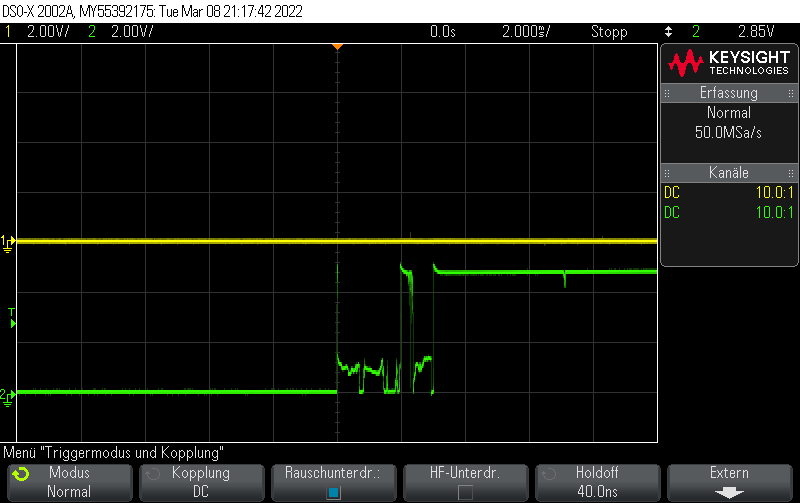
\includegraphics[width=\textwidth]{scope_12.png}
  \caption{DIP Switch output on switching (yellow).}
  \label{fig:bounce}
\end{figure}
The only notable difference between the two tests is that in the manual test, the output enable signal to the \gls{UART} \gls{IC} was set by hand with a DIP Switch and in the automated test, it was controlled by the output of the \gls{EEPROM}.
When looking at the waveforms of the signal coming from the DIP switch, a bouncing of the trigger can sometimes be observed as shown in \cref{fig:bounce}.
In theory this should not have an effect on the content of the scratch register of the \gls{UART} \gls{IC} as the glitch happens on the output enable input of the \gls{IC}.
However, the datasheet explicitly states a minimum time for a read strobe pulse duration of \qty{80}{\nano\second}.
For this reason, the test adapter was altered to include a low pass filter and schmitt trigger on the \texttt{memRamNOE} and \texttt{memRamNWE} control signals because those are the only control signals which are used asynchronously.
All other control signal are only used in components which do not state a minimum pulse duration for it (only setup and hold times in relation to the rising edge of the clock).
After implementing this fix, the manual test worked perfectly for many read cycles which means that the minimum read pulse duration for the \gls{UART} \gls{IC} needs to be respected.

\begin{figure}[t]
  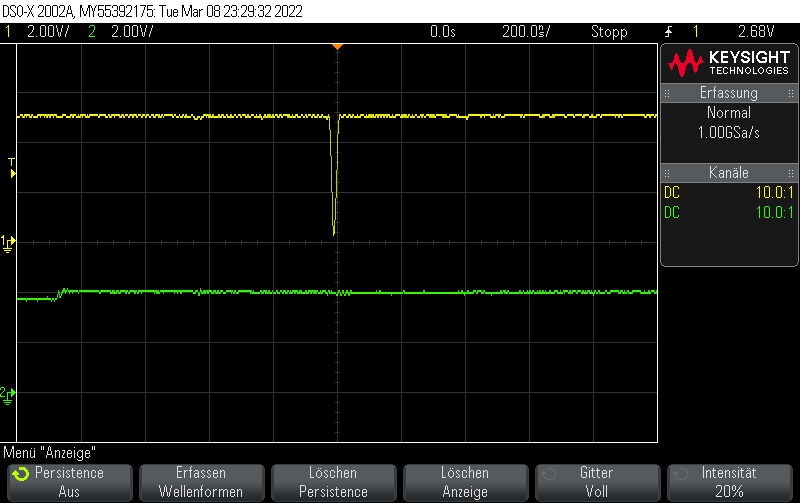
\includegraphics[width=\textwidth]{scope_15.png}
  \caption{Output of the \texttt{memRamNOE} control signal from the \gls{EEPROM} (yellow).}
  \label{fig:EEPROMGlitch}
\end{figure}
Even though, the problem never occurred with the control signals coming from the microcode \gls{EEPROM}, we looked into the specifications for the \gls{EEPROM} and found it also has a period after the address inputs change where the data output is undefined.
When observing the output with the oscilloscope, it was observed that there sometimes are glitches on the \texttt{memRamNOE} control signal as shown in \cref{fig:EEPROMGlitch}.
Therefore, it was decided to add a register to the \texttt{memRamNOE} and \texttt{memRamNWE} control signals.
This results in the microcode needing adjustment to assert these two signals one cycle earlier which was easy to implement and prevented the problem completely.